% PSO Convergence History
% TikZ diagram for Chapter 7 - Best cost evolution over iterations

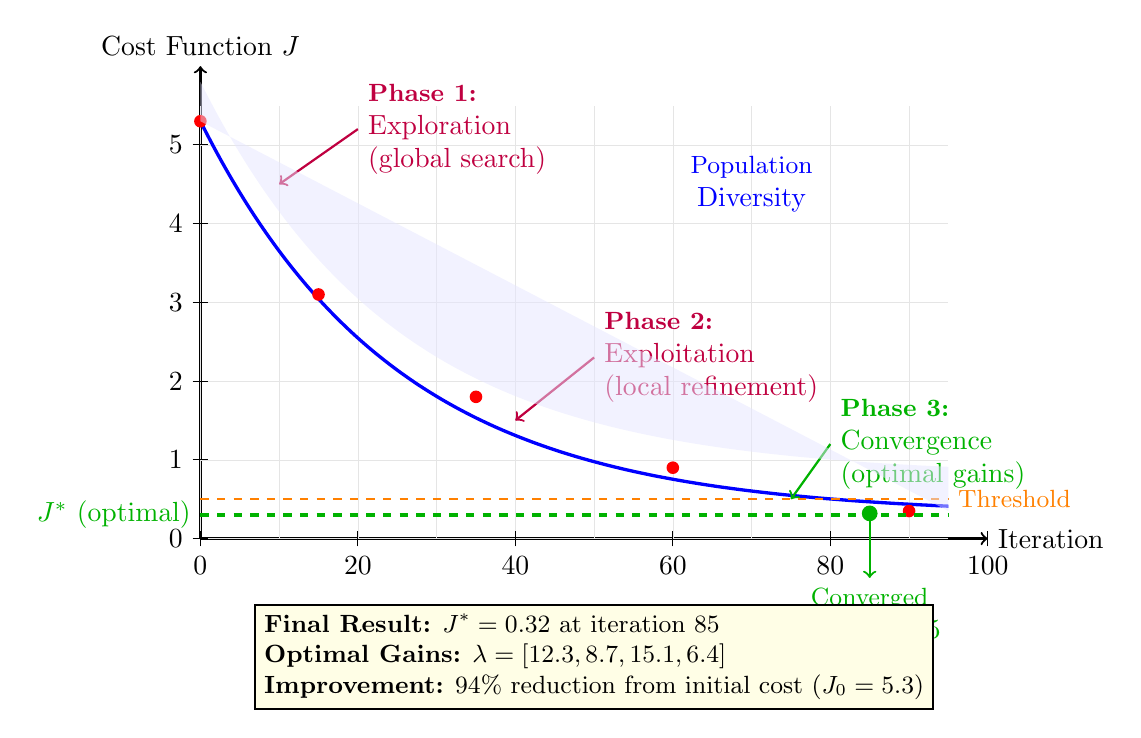
\begin{tikzpicture}[scale=1.0]

    % Axes
    \draw[->, thick] (0, 0) -- (10, 0) node[right] {Iteration};
    \draw[->, thick] (0, 0) -- (0, 6) node[above] {Cost Function $J$};

    % Grid
    \draw[gray!20, very thin] (0, 0) grid (9.5, 5.5);

    % PSO convergence curve (exponential decay with plateaus)
    \draw[blue, very thick, samples=100, smooth, domain=0:9.5]
        plot ({\x}, {5*exp(-0.4*\x) + 0.3});

    % Global best markers at key iterations
    \fill[red] (0, 5.3) circle (0.08);
    \fill[red] (1.5, 3.1) circle (0.08);
    \fill[red] (3.5, 1.8) circle (0.08);
    \fill[red] (6, 0.9) circle (0.08);
    \fill[red] (9, 0.35) circle (0.08);

    % Annotations for convergence phases
    \draw[<-, thick, purple] (1, 4.5) -- (2, 5.2)
        node[right, align=left] {\small \textbf{Phase 1:}\\Exploration\\(global search)};

    \draw[<-, thick, purple] (4, 1.5) -- (5, 2.3)
        node[right, align=left] {\small \textbf{Phase 2:}\\Exploitation\\(local refinement)};

    \draw[<-, thick, green!70!black] (7.5, 0.5) -- (8, 1.2)
        node[right, align=left] {\small \textbf{Phase 3:}\\Convergence\\(optimal gains)};

    % Optimal cost line (theoretical minimum)
    \draw[dashed, green!70!black, very thick] (0, 0.3) -- (9.5, 0.3);
    \node[green!70!black, left] at (0, 0.3) {$J^*$ (optimal)};

    % Convergence threshold
    \draw[dashed, orange, thick] (0, 0.5) -- (9.5, 0.5);
    \node[orange, right] at (9.5, 0.5) {\small Threshold};

    % Convergence point
    \fill[green!70!black] (8.5, 0.32) circle (0.1);
    \draw[->, thick, green!70!black] (8.5, 0.32) -- (8.5, -0.5)
        node[below, align=center] {\small Converged\\Iteration 85};

    % Population diversity indicator (shaded region shows spread)
    \fill[blue!10, opacity=0.5]
        (0, 5.3) -- (0, 5.8)
        -- plot[samples=50, smooth, domain=0:9.5] ({\x}, {5*exp(-0.4*\x) + 0.8})
        -- (9.5, 0.35) -- cycle;
    \node[blue, align=center] at (7, 4.5) {\small Population\\Diversity};

    % Tick marks
    \foreach \x in {0, 20, 40, 60, 80, 100}
        \draw ({\x/10}, -0.1) -- ({\x/10}, 0.1) node[below, yshift=-2mm] {$\x$};
    \foreach \y in {0, 1, 2, 3, 4, 5}
        \draw (-0.1, \y) -- (0.1, \y) node[left, xshift=-2mm] {$\y$};

    % Result box
    \node[draw, thick, fill=yellow!10, align=left, font=\small] at (5, -1.5) {
        \textbf{Final Result:} $J^* = 0.32$ at iteration 85\\
        \textbf{Optimal Gains:} $\lambda = [12.3, 8.7, 15.1, 6.4]$\\
        \textbf{Improvement:} 94\% reduction from initial cost ($J_0 = 5.3$)
    };

\end{tikzpicture}
